\apendice{Especificación de Requisitos}

\section{Introducción}
En este anexo se van a exponer las especificaciones de requisitos que definen el funcionamiento de la plataforma, comenzando por un repaso de objetivos de esta, exponiéndose los requisitos funcionales y no funcionales derivados de estos y finalizando con la exposición de los casos de uso resultantes de su desarrollo.

\section{Objetivos generales}
Como había sido mencionado previamente en la memoria, el objetivo principal de este proyecto consistía en el desarrollo de una plataforma web orientada a la enseñanza online la cual permita corregir de forma automática ejercicios en Python. Para ello, la plataforma debía basarse en la inclusión de cursos de carácter didáctico por parte de los profesores en los que se encontrarían las tareas y los contenidos teóricos de estos.

\newpage

\section{Catálogo de requisitos}
En esta sección son enumerados y descritos los requisitos funcionales y no funcionales derivados del objetivo descrito con anterioridad.

\subsection{Requisitos funcionales de un usuario sin autenticar:}
\begin{itemize}
\tightlist
\item
  \textbf{RF-1 Inicio de sesión:} Un usuario inicia sesión en la plataforma y es identificado
  como profesor o estudiante y llevado a la página principal correspondiente.
  
\end{itemize}

\subsection{Requisitos funcionales orientados al profesor:}
\begin{itemize}
\tightlist

\item
  \textbf{RF-2 Gestionar cursos:} Un profesor debe poder realizar la gestión de sus cursos.
  
  \begin{itemize}
  \tightlist
  \item
    \textbf{RF-2.1 Gestionar contenidos de un curso:} Un profesor debe poder gestionar los contenidos de cada curso.

    \begin{itemize}
    \tightlist
    \item
      \textbf{RF-2.1.1: Descargar contenidos y tareas:} Un profesor debe poder descargar los contenidos teóricos y tareas tanto en versión alumno como versión profesor de las secciones contenidas en el curso.
      
    \item  
      \textbf{RF-2.1.2: Gestionar secciones no publicadas:} Un profesor debe poder acceder a la gestión de las secciones no publicadas de ese curso.
      
      \begin{itemize}
      \tightlist
      \item
        \textbf{RF-2.1.2.1: Crear sección no publicada:} Un profesor debe poder crear nuevas secciones no publicadas para un curso.
        
      \item
        \textbf{RF-2.1.2.2: Editar tarea:} Un profesor debe poder editar las tareas de las secciones no publicada desde la propia plataforma.
        
      \item
        \textbf{RF-2.1.2.3: Descargar estado de la tarea:} Un profesor debe poder descargarse el estado actual en el que se encuentran las tareas de las seccies no publicadas.
        
      \item
        \textbf{RF-2.1.2.4: Eliminar sección no publicada:} Un profesor debe poder eliminar secciones no publicadas.
        
      \item
        \textbf{RF-2.1.2.5: Publicar sección no publicada:} Un profesor debe poder publicar secciones no publicadas.
      
      \end{itemize}
    
    \item  
      \textbf{RF-2.1.3: Eliminar sección de contenido:} Un profesor debe poder eliminar secciones de contenido ya publicadas de un curso.
      
    \item  
      \textbf{RF-2.1.4: Añadir sección de contenido:} Un profesor debe poder crear secciones de contenido de forma directa.
      
    \end{itemize}
    
  \item
    \textbf{RF-2.2 Gestionar alumnos del curso:} Un profesor debe poder realizar la gestión de alumnos integrantes en cada curso.
    
    \begin{itemize}
    \tightlist
    \item
      \textbf{RF-2.2.1: Quitar alumno de un curso:} Un profesor podrá quitar alumnos de un curso.
        
    \item
      \textbf{RF-2.2.2: Añadir alumno a un curso:} Un profesor podrá añadir alumnos a un curso.
    \end{itemize}
    
  \item
    \textbf{RF-2.3 Crear curso:} Un profesor podrá crear un curso nuevo.
    
  \item
    \textbf{RF-2.4 Eliminar curso:} Un profesor podrá eliminar un curso existente.
    
  \end{itemize}
  
  \item
    \textbf{RF-3 Gestionar alumnos:} Un profesor debe poder acceder a la gesión de alumnos integrantes en sus cursos.
    
    \begin{itemize}
    \tightlist
    \item
      \textbf{RF-3.1: Crear alumno:} Un profesor podrá crear un nuevo alumno, integrándolo en un curso.
        
    \item
      \textbf{RF-3.2: Borrar alumno:} Un profesor podrá eliminar por completo un alumno.
      
    \item
      \textbf{RF-3.3: Acceder a calificaciones del alumno:} Un profesor podrá acceder a la visualización de calificaciones de un alumno en particular.
      
      \begin{itemize}
      \tightlist
      \item
        \textbf{RF-3.3.1: Eliminar entregas:} Un profesor podrá eliminar entregas de tareas de un alumno desde la vista de sus calificaciones.
        
      \item
        \textbf{RF-3.3.2: Descargar feedbacks:} Un profesor podrá descargarse los archivos feedback de cada entrega / calificación de un alumno.
        
      \item
        \textbf{RF-3.3.3: Descargar entregas:} Un profesor podrá descargarse los archivos tarea de cada entrega / calificación de un alumno.
      
      \end{itemize}
      
    \end{itemize}
    
  \item
    \textbf{RF-4 Consultar todas las calificaciones:} Un profesor podrá acceder a la visualización total de las calificaciones de los alumnos pertenecientes a sus cursos.
    
    \begin{itemize}
      \tightlist
      \item
        \textbf{RF-4.1: Descargar feedbacks:} Un profesor podrá descargarse los archivos feedback de cada entrega / calificación de todas las entregas de sus alumnos.
        
      \item
        \textbf{RF-4.2: Descargar entregas:} Un profesor podrá descargarse los archivos tarea de cada entrega / calificación de todas las entregas de sus alumnos.
      
    \end{itemize}

\end{itemize}
 
\subsection{Requisitos funcionales orientados al alumno:}
\begin{itemize}
\tightlist
\item
  \textbf{RF-5 Acceder a cursos inscrito:} Un alumno debe poder acceder al listado de cursos a los que está inscrito.
  
  \begin{itemize}
  \tightlist
  \item
    \textbf{RF-5.1 Acceder a los contenidos de un curso:} Un alumno debe poder acceder a los contenidos de cada uno de los cursos a los que está inscrito.
    
    \begin{itemize}
    \tightlist
    \item
      \textbf{RF-5.1.1 Descargar contenidos y tareas:} Un alumno debe poder descargarse los contenidos teóricos y tareas de cada sección de contenido de un curso.

    \item
      \textbf{RF-5.1.2 Entregar tareas:} Un alumno debe poder realizar la entrega de tareas de las secciones de un curso.
      
    \item
      \textbf{RF-5.1.3 Descargar entregas:} Un alumno debe poder descargarse las entregas previamente realizadas de las secciones de un curso.
  
    \end{itemize}

  \item
    \textbf{RF-5.2 Consultar calificaciones de un curso:} Un alumno debe poder consultar sus calificaciones obtenidas en las tareas de un curso en particular.
    
    \begin{itemize}
    \tightlist
    \item
      \textbf{RF-5.2.1 Descargar entregas:} Un alumno debe poder descargarse el archivo tarea enviado en cada entrega / calificación de un curso.

    \item
      \textbf{RF-5.2.2 Descargar feedbacks:} Un alumno debe poder descargarse el archivo feedback obtenido en cada entrega / calificación de un curso.
  
    \end{itemize}
  
  \end{itemize}
  
\item
    \textbf{RF-6 Consultar todas mis calificaciones:} Un alumno debe poder consultar la totalidad de sus calificaciones obtenidas en todos los cursos a los que está inscrito.
    
    \begin{itemize}
    \tightlist
    \item
      \textbf{RF-6.1 Descargar entregas:} Un alumno debe poder descargarse el archivo tarea enviado en cada entrega / calificación.

    \item
      \textbf{RF-6.2 Descargar feedbacks:} Un alumno debe poder descargarse el archivo feedback obtenido en cada entrega / calificación.
  
    \end{itemize}

\end{itemize}
 
\subsection{Requisitos funcionales comunes a profesores y alumnos:}
\begin{itemize}
\tightlist
\item
  \textbf{RF-7 Cambio de contraseña:} Un usuario profesor o alumno debe poder realizar el cambio de contraseña de su cuenta.
  
\item
  \textbf{RF-8 Cierre de sesión:} Un usuario profesor o alumno debe poder realizar el cierre de sesión de su cuenta.
  
\end{itemize}


\subsection{Requisitos no funcionales:}

\begin{itemize}
\tightlist
	\item \textbf{RNF.1 Usabilidad} El diseño de la plataforma busca la facilidad de uso e intuitividad.
	\item \textbf{RNF.2 Disponibilidad} La aplicación siempre ha de estar disponible para su uso, siempre y cuando se tenga coñexión a internet.
	\item \textbf{RNF.3 Seguridad} Los datos sensibles pertenecientes a los usuarios permanecen aislados en todo momento.
	\item \textbf{RNF.4 Mantenibilidad} El diseño de la platagorma permite una adecuada mantenibilidad.
	\item \textbf{RNF.5 Escalabilidad} La adición de nuevas funcionales es posible y sencillo de realizar.
	
\end{itemize}

\newpage
\section{Especificación de requisitos}

En esta sección son incluidos los diagramas de casos de uso para usuarios sin autenticar, profesores y alumnos y el desarrollo de cada uno de ellos:

\subsection{Diagramas de casos de uso}
\begin{figure}[H]
    \centering
    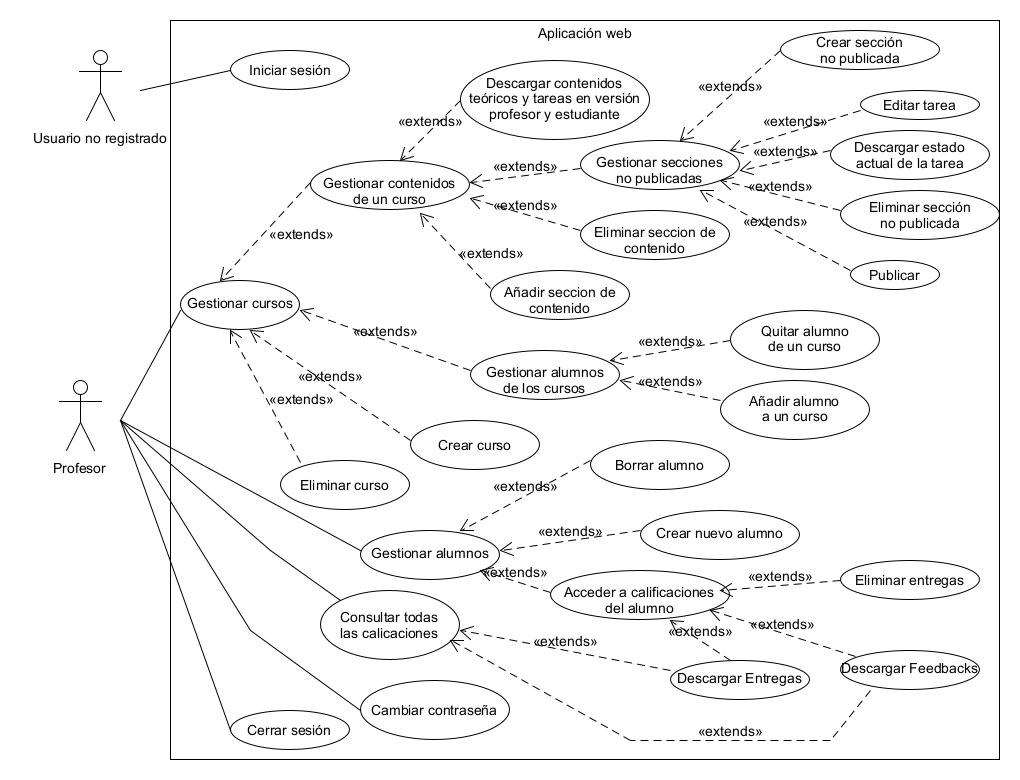
\includegraphics[width=\textwidth]{img/imgs-memoria/CasosDeUso_Profesor.png}
    \caption{Casos de Uso Profesor e Inicio de sesión}
\end{figure}

\begin{figure}[H]
    \centering
    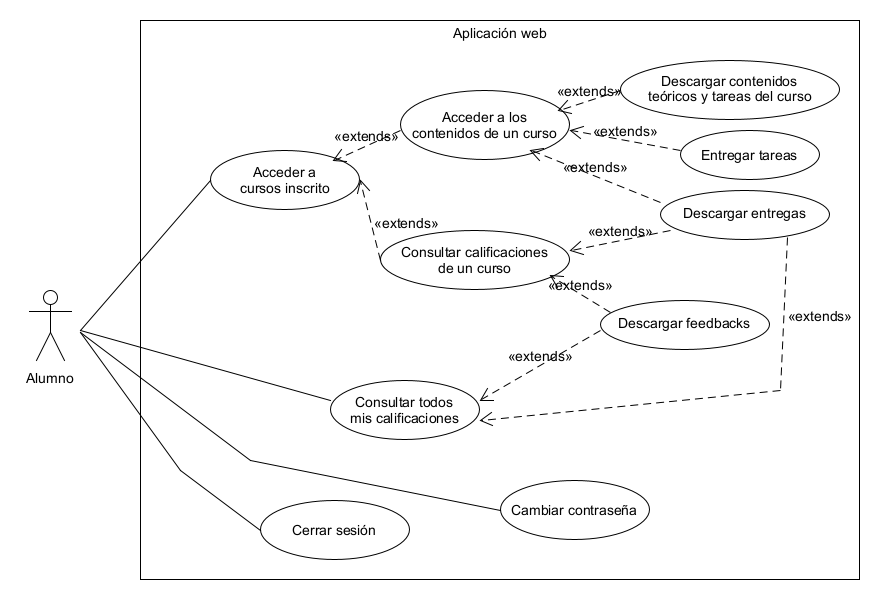
\includegraphics[width=\textwidth]{img/imgs-memoria/CasosDeUso_Alumno.png}
    \caption{Casos de Uso Alumno}
\end{figure}


\newpage
\subsection{Casos de uso}

\begin{adjustwidth}{-2cm}{}
\begin{tabular}[H]{l c l}
\toprule 
\multicolumn{3}{l}{\textbf{Caso de uso 1: Inicio de sesión}}\\
\midrule
Descripción & \multicolumn{2}{p{10cm}}{Permite a un usuario sin autenticar inciar sesión en la plataforma}\\
\midrule
Requisitos relacionados & \multicolumn{2}{p{10cm}}{RF-1}\\
\midrule
Precondiciones & \multicolumn{2}{p{10cm}}{El usuario dispone de una cuenta en la plataforma }\\
\midrule
Secuencia & Paso & Acción \\
\cmidrule{2-3}
         & 1 & El usuario accede al login de la plataforma \\
         & 2 & El usuario introduce su usuario y contraseña\\
         & 3 & Se inicia sesión\\
\midrule
Postcondiciones & \multicolumn{2}{p{10cm}}{El usuario es llevado a la página principal ''Inicio'' correspondiente en caso de ser un alumno o un profesor}\\
\midrule
Excepciones & \multicolumn{2}{p{10cm}}{Datos erróneos}\\
            & \multicolumn{2}{p{10cm}}{La cuenta no existe}\\
\bottomrule 
\end{tabular}


\hspace{3cm}

\begin{tabular}[H]{l c l}
\toprule 
\multicolumn{3}{l}{\textbf{Caso de uso 2: Gestionar cursos}}\\
\midrule
Descripción & \multicolumn{2}{p{10cm}}{Permite a un profesor realizar la gestión de sus cursos}\\
\midrule
Requisitos relacionados & \multicolumn{2}{p{10cm}}{RF-2, RF-2.1, RF-2.1.1, RF-2.1.2, RF-2.1.2.1, RF-2.1.2.2, RF-2.1.2.3
RF-2.1.2.4, RF-2.1.2.5, RF-2.1.3, RF-2.1.4, RF-2.2, RF-2.2.1, RF-2.2.2,  RF-2.3,  RF-2.4}\\
\midrule
Precondiciones & \multicolumn{2}{p{10cm}}{El profesor ha iniciado sesión}\\
\midrule
Secuencia & Paso & Acción \\
\cmidrule{2-3}
         & 1 & \multicolumn{1}{p{8cm}}{El profesor accede a la página de ''cursos'' desde la barra navegacional o desde el botón de ''cursos'' de la página principal ''Inicio''} \\
\midrule
Postcondiciones & \multicolumn{2}{p{10cm}}{El profesor es llevado a la página de gestión de sus cursos ''cursos''}\\
\bottomrule 
\end{tabular}
\end{adjustwidth}

\hspace{3cm}

\begin{tabular}[H]{l c l}
\toprule 
\multicolumn{3}{l}{\textbf{Caso de uso 2.1: Gestionar contenidos de un curso}}\\
\midrule
Descripción & \multicolumn{2}{p{10cm}}{Permite a un profesor realizar la gestión de contenidos de un curso en particular}\\
\midrule
Requisitos relacionados & \multicolumn{2}{p{10cm}}{RF-2, RF-2.1, RF-2.1.1, RF-2.1.2, RF-2.1.2.1, RF-2.1.2.2, RF-2.1.2.3
RF-2.1.2.4, RF-2.1.2.5, RF-2.1.3, RF-2.1.4}\\
\midrule
Precondiciones & \multicolumn{2}{p{10cm}}{El profesor ha accedido a la vista de gestión de cursos y el curso existe}\\
\midrule
Secuencia & Paso & Acción \\
\cmidrule{2-3}
         & 1 &  \multicolumn{1}{p{8cm}}{El profesor hace click en el botón ''Acceder'' del curso del cual quiere hacer la gestión de contenidos}\\

\midrule
Postcondiciones & \multicolumn{2}{p{10cm}}{El profesor es llevado a la página de contenidos del curso en particular}\\
\midrule
Excepciones & \multicolumn{2}{p{10cm}}{El curso no existe}\\
\bottomrule 
\end{tabular}

\hspace{3cm}


\begin{tabular}[H]{l c l}
\toprule 
\multicolumn{3}{l}{\textbf{Caso de uso 2.1.1: Descargar contenidos y tareas}}\\
\midrule
Descripción & \multicolumn{2}{p{10cm}}{Permite a un profesor descargar los archivos de contenidos teóricos y tareas de las secciones de contenido del curso actual }\\
\midrule
Requisitos relacionados & \multicolumn{2}{p{10cm}}{RF-2, RF-2.1, RF-2.1.2, RF-2.1.2.1, RF-2.1.2.2, RF-2.1.2.3
RF-2.1.2.4, RF-2.1.2.5}\\
\midrule
Precondiciones & \multicolumn{2}{p{10cm}}{El profesor ha accedido a la vista de contenidos de un curso}\\
\midrule
Secuencia & Paso & Acción \\
\cmidrule{2-3}
         & 1 &  \multicolumn{1}{p{8cm}}{El profesor hace click en los botones de descarga de contenidos teóricos y tareas de las secciones del curso}\\
\midrule
Postcondiciones & \multicolumn{2}{p{10cm}}{El profesor recibe los archivos que ha solicitado descargar}\\
\midrule
Excepciones & \multicolumn{2}{p{10cm}}{La sección no existe}\\
\bottomrule 
\end{tabular}

\hspace{3cm}

\begin{adjustwidth}{-2cm}{}
\begin{tabular}[H]{l c l}
\toprule 
\multicolumn{3}{l}{\textbf{Caso de uso 2.1.2: Gestionar secciones no publicadas}}\\
\midrule
Descripción & \multicolumn{2}{p{10cm}}{Permite a un profesor realizar la gestión de secciones de contenidos no publicadas de un curso }\\
\midrule
Requisitos relacionados & \multicolumn{2}{p{10cm}}{RF-2, RF-2.1, RF-2.1.2, RF-2.1.2.1, RF-2.1.2.2, RF-2.1.2.3
RF-2.1.2.4, RF-2.1.2.5}\\
\midrule
Precondiciones & \multicolumn{2}{p{10cm}}{El profesor ha accedido a la vista de contenidos de un curso}\\
\midrule
Secuencia & Paso & Acción \\
\cmidrule{2-3}
         & 1 &  \multicolumn{1}{p{8cm}}{El profesor hace click en el botón de acceso a las secciones no publicadas del curso}\\
\midrule
Postcondiciones & \multicolumn{2}{p{10cm}}{El profesor es llevado a la página de secciones no publicadas del curso actual}\\
\bottomrule 
\end{tabular}

\hspace{3cm}

\begin{tabular}[H]{l c l}
\toprule 
\multicolumn{3}{l}{\textbf{Caso de uso 2.1.2.1: Crear sección no publicada}}\\
\midrule
Descripción & \multicolumn{2}{p{10cm}}{Permite a un profesor crear una nueva sección no publicada en el curso actual}\\
\midrule
Requisitos relacionados & \multicolumn{2}{p{10cm}}{RF-2, RF-2.1, RF-2.1.2, RF-2.1.2.1}\\
\midrule
Precondiciones & \multicolumn{2}{p{10cm}}{El profesor ha accedido a la vista de contenidos de un curso o a la vista de secciones no publicadas de ese curso}\\
\midrule
Secuencia & Paso & Acción \\
\cmidrule{2-3}
         & 1 &  \multicolumn{1}{p{8cm}}{El profesor hace click en el botón de creación de sección no publicadas desde la vista del curso o la vista de secciones no publicadas del curso}\\
\midrule
Postcondiciones & \multicolumn{2}{p{10cm}}{Es creada una nueva sección no publicada y aparecerá en la vista de secciones no publicadas del curso}\\
\midrule
Excepciones & \multicolumn{2}{p{10cm}}{Información necesaria no aportada}\\
            & \multicolumn{2}{p{10cm}}{Contenidos pertenecientes a otra sección}\\
\bottomrule 
\end{tabular}
\end{adjustwidth}
\hspace{3cm}


\begin{tabular}[H]{l c l}
\toprule 
\multicolumn{3}{l}{\textbf{Caso de uso 2.1.2.2: Editar tarea}}\\
\midrule
Descripción & \multicolumn{2}{p{10cm}}{Permite a un profesor editar la tarea de una sección no publicada}\\
\midrule
Requisitos relacionados & \multicolumn{2}{p{10cm}}{RF-2, RF-2.1, RF-2.1.2, RF-2.1.2.2}\\
\midrule
Precondiciones & \multicolumn{2}{p{10cm}}{El profesor ha accedido a la vista de secciones no publicadas de ese curso}\\
\midrule
Secuencia & Paso & Acción \\
\cmidrule{2-3}
         & 1 &  \multicolumn{1}{p{8cm}}{El profesor hace click en el botón edición de tarea de una sección no publicada}\\
         & 2 &  \multicolumn{1}{p{8cm}}{El profesor edita la tarea desde la vista del notebook tarea que es abierta al realizar el paso anterior}\\
         & 3 &  \multicolumn{1}{p{8cm}}{El profesor guarda los cambios en el botón de guardado del notebook}\\
\midrule
Postcondiciones & \multicolumn{2}{p{10cm}}{La tarea es editada}\\
\midrule
Excepciones & \multicolumn{2}{p{10cm}}{La sección no publicada no existe}\\
\bottomrule 
\end{tabular}

\hspace{3cm}


\begin{tabular}[H]{l c l}
\toprule 
\multicolumn{3}{l}{\textbf{Caso de uso 2.1.2.3: Descargar estado de la tarea}}\\
\midrule
Descripción & \multicolumn{2}{p{10cm}}{Permite a un profesor descargar el estado actual de las tareas de las secciones no publicadas}\\
\midrule
Requisitos relacionados & \multicolumn{2}{p{10cm}}{RF-2, RF-2.1, RF-2.1.2, RF-2.1.2.3}\\
\midrule
Precondiciones & \multicolumn{2}{p{10cm}}{El profesor ha accedido a la vista de secciones no publicadas de ese curso}\\
\midrule
Secuencia & Paso & Acción \\
\cmidrule{2-3}
         & 1 &  \multicolumn{1}{p{8cm}}{El profesor hace click en el botón de descarga de la tarea de una sección no publicada}\\

\midrule
Postcondiciones & \multicolumn{2}{p{10cm}}{El profesor recibe el notebook tarea seleccionado}\\
\midrule
Excepciones & \multicolumn{2}{p{10cm}}{La sección no publicada no existe}\\
\bottomrule 
\end{tabular}

\hspace{3cm}

\begin{adjustwidth}{-2cm}{}
\begin{tabular}[H]{l c l}
\toprule 
\multicolumn{3}{l}{\textbf{Caso de uso 2.1.2.4: Eliminar sección no publicada}}\\
\midrule
Descripción & \multicolumn{2}{p{10cm}}{Permite a un profesor eliminar secciones no publicadas}\\
\midrule
Requisitos relacionados & \multicolumn{2}{p{10cm}}{RF-2, RF-2.1, RF-2.1.2, RF-2.1.2.4}\\
\midrule
Precondiciones & \multicolumn{2}{p{10cm}}{El profesor ha accedido a la vista de secciones no publicadas de ese curso}\\
\midrule
Secuencia & Paso & Acción \\
\cmidrule{2-3}
         & 1 &  \multicolumn{1}{p{8cm}}{El profesor hace click en el botón de eliminación de una sección no publicada}\\
         & 2 &  \multicolumn{1}{p{8cm}}{El profesor hace click en el botón de confirmación del modal emergente}\\
\midrule
Postcondiciones & \multicolumn{2}{p{10cm}}{La sección no publicada es eliminada}\\
\midrule
Excepciones & \multicolumn{2}{p{10cm}}{La sección no publicada no existe}\\
\bottomrule 
\end{tabular}

\hspace{3cm}

\begin{tabular}[H]{l c l}
\toprule 
\multicolumn{3}{l}{\textbf{Caso de uso 2.1.2.5: Publicar sección no publicada}}\\
\midrule
Descripción & \multicolumn{2}{p{10cm}}{Permite a un profesor publicar secciones no publicadas}\\
\midrule
Requisitos relacionados & \multicolumn{2}{p{10cm}}{RF-2, RF-2.1, RF-2.1.2, RF-2.1.2.5}\\
\midrule
Precondiciones & \multicolumn{2}{p{10cm}}{El profesor ha accedido a la vista de secciones no publicadas de ese curso}\\
\midrule
Secuencia & Paso & Acción \\
\cmidrule{2-3}
         & 1 &  \multicolumn{1}{p{8cm}}{El profesor hace click en el botón de publicación de una sección no publicada}\\
         & 2 &  \multicolumn{1}{p{8cm}}{El profesor hace click en el botón de confirmación del modal emergente}\\

\midrule
Postcondiciones & \multicolumn{2}{p{10cm}}{La sección no publicada es publicada, aparecerá en la vista de contenido del curso y se genera el archivo tarea correspondiente a esa sección para los alumnos}\\
\midrule
Excepciones & \multicolumn{2}{p{10cm}}{La sección no publicada no existe}\\
\bottomrule 
\end{tabular}
\end{adjustwidth}

\hspace{3cm}

\begin{tabular}[H]{l c l}
\toprule 
\multicolumn{3}{l}{\textbf{Caso de uso 2.1.3: Eliminar seccion de contenido}}\\
\midrule
Descripción & \multicolumn{2}{p{10cm}}{Permite a un profesor eliminar secciones de contenido del curso actual }\\
\midrule
Requisitos relacionados & \multicolumn{2}{p{10cm}}{RF-2, RF-2.1, RF-2.1.3}\\
\midrule
Precondiciones & \multicolumn{2}{p{10cm}}{El profesor ha accedido a la vista de contenidos de un curso}\\
\midrule
Secuencia & Paso & Acción \\
\cmidrule{2-3}
         & 1 &  \multicolumn{1}{p{8cm}}{El profesor hace click en el botón de eliminación de una sección de contenido del curso}\\
         & 2 &  \multicolumn{1}{p{8cm}}{El profesor hace click en el botón de confirmación del modal emergente}\\
         
\midrule
Postcondiciones & \multicolumn{2}{p{10cm}}{La sección de contenido es eliminada}\\
\midrule
Excepciones & \multicolumn{2}{p{10cm}}{La sección no existe}\\
\bottomrule 
\end{tabular}

\hspace{3cm}


\begin{tabular}[H]{l c l}
\toprule 
\multicolumn{3}{l}{\textbf{Caso de uso 2.1.4: Eliminar seccion de contenido}}\\
\midrule
Descripción & \multicolumn{2}{p{10cm}}{Permite a un profesor crear una sección de contenido de forma directa}\\
\midrule
Requisitos relacionados & \multicolumn{2}{p{10cm}}{RF-2, RF-2.1, RF-2.1.4}\\
\midrule
Precondiciones & \multicolumn{2}{p{10cm}}{El profesor ha accedido a la vista de contenidos de un curso}\\
\midrule
Secuencia & Paso & Acción \\
\cmidrule{2-3}
         & 1 &  \multicolumn{1}{p{8cm}}{El profesor hace click en el botón de creación de sección de contenido y es llevado a la vista de creación de sección}\\
         & 2 &  \multicolumn{1}{p{8cm}}{El profesor completa el formulario de creación de sección en el que introducirá el archivo de contenido teórico de la sección y el notebook tarea correspondiente a esa sección}\\
         & 3 &  \multicolumn{1}{p{8cm}}{El profesor hace click en el botón de crear}\\
         & 4 &  \multicolumn{1}{p{8cm}}{El profesor hace click en el botón de confirmación del modal emergente}\\
         
\midrule
Postcondiciones & \multicolumn{2}{p{10cm}}{La sección de contenido es creada y se genera el archivo tarea correspondiente a esa sección para los alumnos}\\
\bottomrule 
\end{tabular}

\hspace{3cm}

\begin{adjustwidth}{-2cm}{}
\begin{tabular}[H]{l c l}
\toprule 
\multicolumn{3}{l}{\textbf{Caso de uso 2.2: Gestionar alumnos de un curso}}\\
\midrule
Descripción & \multicolumn{2}{p{10cm}}{Permite a un profesor realizar la gestión de alumnos integrantes de un curso en particular}\\
\midrule
Requisitos relacionados & \multicolumn{2}{p{10cm}}{RF-2, RF-2.2, RF-2.2.1, RF-2.2.2}\\
\midrule
Precondiciones & \multicolumn{2}{p{10cm}}{El profesor ha accedido a la vista de gestión de cursos y el curso existe}\\
\midrule
Secuencia & Paso & Acción \\
\cmidrule{2-3}
         & 1 &  \multicolumn{1}{p{8cm}}{El profesor hace click en el botón de gestión de estudiantes del curso del cual quiere realizar la gestión}\\

\midrule
Postcondiciones & \multicolumn{2}{p{10cm}}{El profesor es llevado a la página de estudiantes integrantes y no integrantes del curso en particular}\\
\midrule
Excepciones & \multicolumn{2}{p{10cm}}{El curso no existe}\\
\bottomrule 
\end{tabular}

\hspace{3cm}

\begin{tabular}[H]{l c l}
\toprule 
\multicolumn{3}{l}{\textbf{Caso de uso 2.2.1: Quitar alumno de un curso}}\\
\midrule
Descripción & \multicolumn{2}{p{10cm}}{Permite a un profesor sacar a un alumno del curso actual}\\
\midrule
Requisitos relacionados & \multicolumn{2}{p{10cm}}{RF-2, RF-2.2, RF-2.2.1}\\
\midrule
Precondiciones & \multicolumn{2}{p{10cm}}{El profesor ha accedido a la vista de estudiantes integrantes y no integrantes del curso en particular}\\
\midrule
Secuencia & Paso & Acción \\
\cmidrule{2-3}
         & 1 &  \multicolumn{1}{p{8cm}}{El profesor hace click en el botón de extracción de un alumno del curso}\\
         & 2 &  \multicolumn{1}{p{8cm}}{El profesor hace click en el botón de confirmación del modal emergente}\\
\midrule
Postcondiciones & \multicolumn{2}{p{10cm}}{El alumno es extraido del curso}\\
\midrule
Excepciones & \multicolumn{2}{p{10cm}}{El alumno no pertenecía al curso}\\
\bottomrule 
\end{tabular}
\end{adjustwidth}


\hspace{3cm}

\begin{tabular}[H]{l c l}
\toprule 
\multicolumn{3}{l}{\textbf{Caso de uso 2.2.2: Añadir alumno a un curso}}\\
\midrule
Descripción & \multicolumn{2}{p{10cm}}{Permite a un profesor añadir a un alumno al curso actual}\\
\midrule
Requisitos relacionados & \multicolumn{2}{p{10cm}}{RF-2, RF-2.2, RF-2.2.2}\\
\midrule
Precondiciones & \multicolumn{2}{p{10cm}}{El profesor ha accedido a la vista de estudiantes integrantes y no integrantes del curso en particular}\\
\midrule
Secuencia & Paso & Acción \\
\cmidrule{2-3}
         & 1 &  \multicolumn{1}{p{8cm}}{El profesor hace click en el botón de adición de un alumno al curso}\\
         & 2 &  \multicolumn{1}{p{8cm}}{El profesor hace click en el botón de confirmación del modal emergente}\\
\midrule
Postcondiciones & \multicolumn{2}{p{10cm}}{El alumno es añadido al curso}\\
\midrule
Excepciones & \multicolumn{2}{p{10cm}}{El alumno ya pertenecía al curso}\\
\bottomrule 
\end{tabular}

\hspace{3cm}

\begin{tabular}[H]{l c l}
\toprule 
\multicolumn{3}{l}{\textbf{Caso de uso 2.3: Crear curso}}\\
\midrule
Descripción & \multicolumn{2}{p{10cm}}{Permite a un profesor crear un nuevo curso}\\
\midrule
Requisitos relacionados & \multicolumn{2}{p{10cm}}{RF-2, RF-2.3}\\
\midrule
Precondiciones & \multicolumn{2}{p{10cm}}{El profesor ha accedido a la vista de gestión de cursos}\\
\midrule
Secuencia & Paso & Acción \\
\cmidrule{2-3}
         & 1 &  \multicolumn{1}{p{8cm}}{El profesor hace click en el botón de creación de un nuevo curso y es llevado a la vista de creación de curso}\\
         & 2 &  \multicolumn{1}{p{8cm}}{El profesor completa el formulario de creación de un curso}\\
         & 3 &  \multicolumn{1}{p{8cm}}{El profesor hace click en el botón de crear curso}\\
         & 4 &  \multicolumn{1}{p{8cm}}{El profesor hace click en el botón de confirmación del modal emergente}\\

\midrule
Postcondiciones & \multicolumn{2}{p{10cm}}{El curso es creado y visualizable en la vista de gestión de cursos}\\
\midrule
Excepciones & \multicolumn{2}{p{10cm}}{Información necesaria no aportada}\\
            & \multicolumn{2}{p{10cm}}{Contenidos pertenecientes a otro curso}\\
\bottomrule 
\end{tabular}

\hspace{3cm}

\begin{adjustwidth}{-2cm}{}
\begin{tabular}[H]{l c l}
\toprule 
\multicolumn{3}{l}{\textbf{Caso de uso 2.4: Eliminar curso}}\\
\midrule
Descripción & \multicolumn{2}{p{10cm}}{Permite a un profesor elimianr un curso}\\
\midrule
Requisitos relacionados & \multicolumn{2}{p{10cm}}{RF-2, RF-2.4}\\
\midrule
Precondiciones & \multicolumn{2}{p{10cm}}{El profesor ha accedido a la vista de gestión de cursos}\\
\midrule
Secuencia & Paso & Acción \\
\cmidrule{2-3}
         & 1 &  \multicolumn{1}{p{8cm}}{El profesor hace click en el botón de eliminación de un curso}\\
         & 2 &  \multicolumn{1}{p{8cm}}{El profesor hace click en el botón de confirmación del modal emergente}\\

\midrule
Postcondiciones & \multicolumn{2}{p{10cm}}{El curso es eliminado}\\
\midrule
Excepciones & \multicolumn{2}{p{10cm}}{El curso no existe}\\
\bottomrule 
\end{tabular}


\hspace{3cm}


\begin{tabular}[H]{l c l}
\toprule 
\multicolumn{3}{l}{\textbf{Caso de uso 3: Gestionar alumnos}}\\
\midrule
Descripción & \multicolumn{2}{p{10cm}}{Permite a un profesor realizar la gestión de alumnos pertenecientes a sus cursos}\\
\midrule
Requisitos relacionados & \multicolumn{2}{p{10cm}}{RF-3, RF-3.1, RF-3.2, RF-3.3, RF-3.3.1, RF-3.3.2, RF-3.3.3}\\
\midrule
Precondiciones & \multicolumn{2}{p{10cm}}{El profesor ha iniciado sesión}\\
\midrule
Secuencia & Paso & Acción \\
\cmidrule{2-3}
         & 1 & \multicolumn{1}{p{8cm}}{El profesor accede a la página de gestión de alumnos desde la barra navegacional o desde el botón de gestión de alumnos de la página principal} \\
\midrule
Postcondiciones & \multicolumn{2}{p{10cm}}{El profesor es llevado a la página de gestión de alumnos}\\
\bottomrule 
\end{tabular}
\end{adjustwidth}

\hspace{3cm}

\begin{tabular}[H]{l c l}
\toprule 
\multicolumn{3}{l}{\textbf{Caso de uso 3.1: Crear alumno}}\\
\midrule
Descripción & \multicolumn{2}{p{10cm}}{Permite a un profesor crear un nuevo alumno}\\
\midrule
Requisitos relacionados & \multicolumn{2}{p{10cm}}{RF-3, RF-3.1}\\
\midrule
Precondiciones & \multicolumn{2}{p{10cm}}{El profesor ha accedido a la vista de gestión de alumnos pertenecientes a sus cursos}\\
\midrule
Secuencia & Paso & Acción \\
\cmidrule{2-3}
         & 1 &  \multicolumn{1}{p{8cm}}{El profesor hace click en el botón de creación de un nuevo alumno y es llevado a la vista de creación de alumno}\\
         & 2 &  \multicolumn{1}{p{8cm}}{El profesor completa el formulario de creación del alumno y selecciona un curso al que quiere ingresar al alumno}\\
         & 3 &  \multicolumn{1}{p{8cm}}{El profesor hace click en el botón de crear alumno}\\
         & 4 &  \multicolumn{1}{p{8cm}}{El profesor hace click en el botón de confirmación del modal emergente}\\

\midrule
Postcondiciones & \multicolumn{2}{p{10cm}}{El alumno es creado y visualizable en la vista de gestión de alumnos}\\
\midrule
Excepciones & \multicolumn{2}{p{10cm}}{Información necesaria no aportada}\\
            & \multicolumn{2}{p{10cm}}{Contenidos pertenecientes a otro alumno}\\
\bottomrule 
\end{tabular}

\hspace{3cm}

\begin{adjustwidth}{-2cm}{}
\begin{tabular}[H]{l c l}
\toprule 
\multicolumn{3}{l}{\textbf{Caso de uso 3.2: Borrar alumno}}\\
\midrule
Descripción & \multicolumn{2}{p{10cm}}{Permite a un profesor borrar un alumno}\\
\midrule
Requisitos relacionados & \multicolumn{2}{p{10cm}}{RF-3, RF-3.2}\\
\midrule
Precondiciones & \multicolumn{2}{p{10cm}}{El profesor ha accedido a la vista de gestión de alumnos pertenecientes a sus cursos}\\
\midrule
Secuencia & Paso & Acción \\
\cmidrule{2-3}
         & 1 &  \multicolumn{1}{p{8cm}}{El profesor hace click en el nombre del estudiante accediendo al perfil este en el que se visualizan las calificaciones}\\
         & 2 &  \multicolumn{1}{p{8cm}}{El profesor hace click en el botón de eliminación del alumno}\\
         & 3 &  \multicolumn{1}{p{8cm}}{El profesor hace click en el botón de confirmación del modal emergente}\\

\midrule
Postcondiciones & \multicolumn{2}{p{10cm}}{El alumno es eliminado junto con su cuenta}\\
\midrule
Excepciones & \multicolumn{2}{p{10cm}}{El alumno no existe}\\
\bottomrule 
\end{tabular}

\hspace{3cm}

\begin{tabular}[H]{l c l}
\toprule 
\multicolumn{3}{l}{\textbf{Caso de uso 3.3: Acceder a las calificaciones de un alumno}}\\
\midrule
Descripción & \multicolumn{2}{p{10cm}}{Permite a un profesor visualizar todas las calificaciones de un alumno en particular}\\
\midrule
Requisitos relacionados & \multicolumn{2}{p{10cm}}{RF-3, RF-3.3, RF-3.3.1, RF-3.3.2,  RF-3.3.3}\\
\midrule
Precondiciones & \multicolumn{2}{p{10cm}}{El profesor ha accedido a la vista de gestión de alumnos pertenecientes a sus cursos}\\
\midrule
Secuencia & Paso & Acción \\
\cmidrule{2-3}
         & 1 &  \multicolumn{1}{p{8cm}}{El profesor hace click en el nombre del estudiante accediendo al perfil este en el que se visualizan las calificaciones}\\

\midrule
Postcondiciones & \multicolumn{2}{p{10cm}}{El profesor visualiza las calificaciones}\\
\midrule
Excepciones & \multicolumn{2}{p{10cm}}{El alumno no existe}\\
\bottomrule 
\end{tabular}
\end{adjustwidth}


\hspace{3cm}


\begin{tabular}[H]{l c l}
\toprule 
\multicolumn{3}{l}{\textbf{Caso de uso 3.3.1: Eliminar entregas}}\\
\midrule
Descripción & \multicolumn{2}{p{10cm}}{Permite a un profesor eliminar entregas / calificaciones de tareas realizadas por un alumno en particular}\\
\midrule
Requisitos relacionados & \multicolumn{2}{p{10cm}}{RF-3, RF-3.3, RF-3.3.1}\\
\midrule
Precondiciones & \multicolumn{2}{p{10cm}}{El profesor ha accedido a la vista de gestión de alumnos pertenecientes a sus cursos}\\
\midrule
Secuencia & Paso & Acción \\
\cmidrule{2-3}
         & 1 &  \multicolumn{1}{p{8cm}}{El profesor hace click en el nombre del estudiante accediendo al perfil este en el que se visualizan las calificaciones}\\
         & 2 &  \multicolumn{1}{p{8cm}}{El profesor hace click en el botón de eliminación de entrega de una calificación en particular}\\
         & 3 &  \multicolumn{1}{p{8cm}}{El profesor hace click en el botón de confirmación del modal emergente}\\
\midrule
Postcondiciones & \multicolumn{2}{p{10cm}}{El profesor elimina la entrega}\\
\midrule
Excepciones & \multicolumn{2}{p{10cm}}{La calificación no existe}\\
\bottomrule 
\end{tabular}

\hspace{3cm}

\begin{tabular}[H]{l c l}
\toprule 
\multicolumn{3}{l}{\textbf{Caso de uso 3.3.2: Descargar feedback}}\\
\midrule
Descripción & \multicolumn{2}{p{10cm}}{Permite a un profesor descargar los archivos de feedback de las entregas / calificaciones de un alumno en particular}\\
\midrule
Requisitos relacionados & \multicolumn{2}{p{10cm}}{RF-3, RF-3.3, RF-3.3.2}\\
\midrule
Precondiciones & \multicolumn{2}{p{10cm}}{El profesor ha accedido a la vista de gestión de alumnos pertenecientes a sus cursos}\\
\midrule
Secuencia & Paso & Acción \\
\cmidrule{2-3}
         & 1 &  \multicolumn{1}{p{8cm}}{El profesor hace click en el nombre del estudiante accediendo al perfil este en el que se visualizan las calificaciones}\\
         & 2 &  \multicolumn{1}{p{8cm}}{El profesor hace click en el botón de descarga de feedback de una calificación en particular}\\

\midrule
Postcondiciones & \multicolumn{2}{p{10cm}}{El profesor recibe el archivo feedback}\\
\midrule
Excepciones & \multicolumn{2}{p{10cm}}{La calificación no existe}\\
\bottomrule 
\end{tabular}

\hspace{3cm}

\begin{adjustwidth}{-2cm}{}
\begin{tabular}[H]{l c l}
\toprule 
\multicolumn{3}{l}{\textbf{Caso de uso 3.3.3: Descargar entregas}}\\
\midrule
Descripción & \multicolumn{2}{p{10cm}}{Permite a un profesor descargar los archivos entregados de las entregas / calificaciones de un alumno en particular}\\
\midrule
Requisitos relacionados & \multicolumn{2}{p{10cm}}{RF-3, RF-3.3, RF-3.3.3}\\
\midrule
Precondiciones & \multicolumn{2}{p{10cm}}{El profesor ha accedido a la vista de gestión de alumnos pertenecientes a sus cursos}\\
\midrule
Secuencia & Paso & Acción \\
\cmidrule{2-3}
         & 1 &  \multicolumn{1}{p{8cm}}{El profesor hace click en el nombre del estudiante accediendo al perfil este en el que se visualizan las calificaciones}\\
         & 2 &  \multicolumn{1}{p{8cm}}{El profesor hace click en el botón de descarga de entrega de una calificación en particular}\\

\midrule
Postcondiciones & \multicolumn{2}{p{10cm}}{El profesor recibe el archivo de entrega del alumno}\\
\midrule
Excepciones & \multicolumn{2}{p{10cm}}{La calificación no existe}\\
\bottomrule 
\end{tabular}

\hspace{3cm} 

\begin{tabular}[H]{l c l}
\toprule 
\multicolumn{3}{l}{\textbf{Caso de uso 4: Consultar todas las calificaciones}}\\
\midrule
Descripción & \multicolumn{2}{p{10cm}}{Permite a un profesor acceder a todas las calificaciones de todos los alumnos pertenecientes a sus cursos}\\
\midrule
Requisitos relacionados & \multicolumn{2}{p{10cm}}{RF-4, RF-4.1, RF-4.2}\\
\midrule
Precondiciones & \multicolumn{2}{p{10cm}}{El profesor ha iniciado sesión}\\
\midrule
Secuencia & Paso & Acción \\
\cmidrule{2-3}
         & 1 & \multicolumn{1}{p{8cm}}{El profesor accede a la página de calificaciones desde la barra navegacional o desde el botón de calificaciones de la página principal} \\
\midrule
Postcondiciones & \multicolumn{2}{p{10cm}}{El profesor es llevado a la página de calificaciones}\\
\bottomrule 
\end{tabular}
\end{adjustwidth}


\hspace{3cm} 

\begin{tabular}[H]{l c l}
\toprule 
\multicolumn{3}{l}{\textbf{Caso de uso 4.1: Descargar feedback}}\\
\midrule
Descripción & \multicolumn{2}{p{10cm}}{Permite a un profesor descargar los archivos de feedback de las entregas / calificaciones de sus alumnos}\\
\midrule
Requisitos relacionados & \multicolumn{2}{p{10cm}}{RF-4, RF-4.1}\\
\midrule
Precondiciones & \multicolumn{2}{p{10cm}}{El profesor ha accedido a la vista de calificaciones}\\
\midrule
Secuencia & Paso & Acción \\
\cmidrule{2-3}
         & 1 &  \multicolumn{1}{p{8cm}}{El profesor hace click en el botón de descarga de feedback de una calificación en particular}\\
\midrule
Postcondiciones & \multicolumn{2}{p{10cm}}{El profesor recibe el archivo feedback}\\
\midrule
Excepciones & \multicolumn{2}{p{10cm}}{La calificación no existe}\\
\bottomrule 
\end{tabular}



\hspace{3cm} 


\begin{tabular}[H]{l c l}
\toprule 
\multicolumn{3}{l}{\textbf{Caso de uso 4.2: Descargar entregas}}\\
\midrule
Descripción & \multicolumn{2}{p{10cm}}{Permite a un profesor descargar los archivos entregados de las entregas / calificaciones de sus alumnos}\\
\midrule
Requisitos relacionados & \multicolumn{2}{p{10cm}}{RF-4, RF-4.2}\\
\midrule
Precondiciones & \multicolumn{2}{p{10cm}}{El profesor ha accedido a la vista de calificaciones}\\
\midrule
Secuencia & Paso & Acción \\
\cmidrule{2-3}
         & 1 &  \multicolumn{1}{p{8cm}}{El profesor hace click en el botón de descarga de entrega de una calificación en particular}\\
\midrule
Postcondiciones & \multicolumn{2}{p{10cm}}{El profesor recibe el archivo de entrega del alumno}\\
\midrule
Excepciones & \multicolumn{2}{p{10cm}}{La calificación no existe}\\
\bottomrule 
\end{tabular}

\hspace{3cm} 


\begin{adjustwidth}{-2cm}{}
\begin{tabular}[H]{l c l}
\toprule 
\multicolumn{3}{l}{\textbf{Caso de uso 5: Acceder a cursos inscrito}}\\
\midrule
Descripción & \multicolumn{2}{p{10cm}}{Permite a un alumno acceder a los cursos a los que está inscrito}\\
\midrule
Requisitos relacionados & \multicolumn{2}{p{10cm}}{RF-5, RF-5.1, RF-5.1.1, RF-5.1.2, RF-5.1.3}\\
\midrule
Precondiciones & \multicolumn{2}{p{10cm}}{El alumno ha iniciado sesión}\\
\midrule
Secuencia & Paso & Acción \\
\cmidrule{2-3}
         & 1 & \multicolumn{1}{p{8cm}}{El alumno accede a la página de cursos desde la barra navegacional o desde el botón de cursos de la página principal} \\
\midrule
Postcondiciones & \multicolumn{2}{p{10cm}}{El alumno es llevado a la página de cursos}\\
\bottomrule 
\end{tabular}


\hspace{3cm} 

\begin{tabular}[H]{l c l}
\toprule 
\multicolumn{3}{l}{\textbf{Caso de uso 5.1: Acceder a contenidos de un curso}}\\
\midrule
Descripción & \multicolumn{2}{p{10cm}}{Permite a un alumno realizar acceder a los contenidos de un curso en particular}\\
\midrule
Requisitos relacionados & \multicolumn{2}{p{10cm}}{RF-5, RF-5.1, RF-5.1.1,  RF-5.1.2, RF-5.1.3}\\
\midrule
Precondiciones & \multicolumn{2}{p{10cm}}{El alumno ha accedido a la vista de cursos y el curso existe}\\
\midrule
Secuencia & Paso & Acción \\
\cmidrule{2-3}
         & 1 &  \multicolumn{1}{p{8cm}}{El alumno hace click en el botón de acceso al curso}\\

\midrule
Postcondiciones & \multicolumn{2}{p{10cm}}{El alumno es llevado a la página de contenidos del curso en particular}\\
\midrule
Excepciones & \multicolumn{2}{p{10cm}}{El curso no existe}\\
\bottomrule 
\end{tabular}
\end{adjustwidth}

\hspace{3cm} 

\begin{tabular}[H]{l c l}
\toprule 
\multicolumn{3}{l}{\textbf{Caso de uso 5.1.1: Descargar contenidos y tareas}}\\
\midrule
Descripción & \multicolumn{2}{p{10cm}}{Permite a un alumno descargarse los contenidos teóricos y tareas de las secciones pertenecientes al curso en particular}\\
\midrule
Requisitos relacionados & \multicolumn{2}{p{10cm}}{RF-5, RF-5.1, RF-5.1.1}\\
\midrule
Precondiciones & \multicolumn{2}{p{10cm}}{El alumno ha accedido a la vista del curso y la sección de contenido existe}\\
\midrule
Secuencia & Paso & Acción \\
\cmidrule{2-3}
         & 1 &  \multicolumn{1}{p{8cm}}{El alumno hace click los botones de descarga de contenido teórico y tareas de la sección en particular de la que quiere obtener los archivos}\\

\midrule
Postcondiciones & \multicolumn{2}{p{10cm}}{El alumno recibe los archivos pedidos}\\
\midrule
Excepciones & \multicolumn{2}{p{10cm}}{La sección de contenido no existe}\\
\bottomrule 
\end{tabular}

\hspace{3cm} 

\begin{tabular}[H]{l c l}
\toprule 
\multicolumn{3}{l}{\textbf{Caso de uso 5.1.2: Entregar tareas}}\\
\midrule
Descripción & \multicolumn{2}{p{10cm}}{Permite a un alumno realizar la entrega de tareas de un curso}\\
\midrule
Requisitos relacionados & \multicolumn{2}{p{10cm}}{RF-5, RF-5.1, RF-5.1.2}\\
\midrule
Precondiciones & \multicolumn{2}{p{10cm}}{El alumno ha accedido a la vista del curso y la sección de contenido existe}\\
\midrule
Secuencia & Paso & Acción \\
\cmidrule{2-3}
         & 1 &  \multicolumn{1}{p{8cm}}{El alumno hace click en el botón de exploración de archivos de la sección de contenido en la que quiere entregar la tarea}\\
         & 2 &  \multicolumn{1}{p{8cm}}{El alumno hace click en el botón de entrega de la tarea}\\
         
\midrule
Postcondiciones & \multicolumn{2}{p{10cm}}{La entrega es realizada, la calificación es calculada y el archivo de feedback es generado}\\
\midrule
Excepciones & \multicolumn{2}{p{10cm}}{La sección de contenido no existe}\\
            & \multicolumn{2}{p{10cm}}{La tarea ya ha sido entregada previamente}\\
\bottomrule 
\end{tabular}

\hspace{3cm}

\begin{adjustwidth}{-2cm}{}
\begin{tabular}[H]{l c l}
\toprule 
\multicolumn{3}{l}{\textbf{Caso de uso 5.1.3: Descargar entregas}}\\
\midrule
Descripción & \multicolumn{2}{p{10cm}}{Permite a un alumno descargar las entregas de las tareas previamente entregadas desde la propia vista del curso}\\
\midrule
Requisitos relacionados & \multicolumn{2}{p{10cm}}{RF-5, RF-5.1, RF-5.1.3}\\
\midrule
Precondiciones & \multicolumn{2}{p{10cm}}{El alumno ha accedido a la vista del curso y la sección de contenido existe y ha sido entregada su tarea}\\
\midrule
Secuencia & Paso & Acción \\
\cmidrule{2-3}
         & 1 &  \multicolumn{1}{p{8cm}}{El alumno hace click en el botón de descarga de la entrega en la sección correspondiente}\\
         
\midrule
Postcondiciones & \multicolumn{2}{p{10cm}}{El alumno recibe el archivo de entrega}\\
\midrule
Excepciones & \multicolumn{2}{p{10cm}}{La sección de contenido no existe}\\
            & \multicolumn{2}{p{10cm}}{La tarea no ha sido entregada}\\
\bottomrule 
\end{tabular}

\hspace{3cm}


\begin{tabular}[H]{l c l}
\toprule 
\multicolumn{3}{l}{\textbf{Caso de uso 5.2: Consultar calificaciones de un curso}}\\
\midrule
Descripción & \multicolumn{2}{p{10cm}}{Permite a un alumno consultar las calificaciones obtenidas en un curso en particular}\\
\midrule
Requisitos relacionados & \multicolumn{2}{p{10cm}}{RF-5, RF-5.2, RF-5.2.1,  RF-5.2.2}\\
\midrule
Precondiciones & \multicolumn{2}{p{10cm}}{El alumno ha accedido a la vista de cursos y el curso existe}\\
\midrule
Secuencia & Paso & Acción \\
\cmidrule{2-3}
         & 1 &  \multicolumn{1}{p{8cm}}{El alumno hace click en el botón de calificaciones del curso}\\

\midrule
Postcondiciones & \multicolumn{2}{p{10cm}}{El alumno es llevado a la página de calificaciones del curso en particular}\\
\midrule
Excepciones & \multicolumn{2}{p{10cm}}{El curso no existe}\\
\bottomrule 
\end{tabular}
\end{adjustwidth}

\hspace{3cm}

\begin{tabular}[H]{l c l}
\toprule 
\multicolumn{3}{l}{\textbf{Caso de uso 5.2.1: Descargar entregas}}\\
\midrule
Descripción & \multicolumn{2}{p{10cm}}{Permite a un alumno descargar las entregas de las tareas previamente entregadas desde la vista de calificaciones de un curso particular}\\
\midrule
Requisitos relacionados & \multicolumn{2}{p{10cm}}{RF-5, RF-5.2, RF-5.2.1}\\
\midrule
Precondiciones & \multicolumn{2}{p{10cm}}{El alumno ha accedido a la vista de calificaciones de un curso particular}\\
\midrule
Secuencia & Paso & Acción \\
\cmidrule{2-3}
         & 1 &  \multicolumn{1}{p{8cm}}{El alumno hace click en el botón de descarga de entrega de una calificación en particular}\\
         
\midrule
Postcondiciones & \multicolumn{2}{p{10cm}}{El alumno recibe el archivo de entrega}\\
\midrule
Excepciones  & \multicolumn{2}{p{10cm}}{La calificación no existe}\\
\bottomrule 
\end{tabular}


\hspace{3cm}

\begin{tabular}[H]{l c l}
\toprule 
\multicolumn{3}{l}{\textbf{Caso de uso 5.2.2: Descargar feedback}}\\
\midrule
Descripción & \multicolumn{2}{p{10cm}}{Permite a un alumno descargar los archivos de feedback de las entregas / calificaciones desde la vista de calificaciones de un curso particular}\\
\midrule
Requisitos relacionados & \multicolumn{2}{p{10cm}}{RF-5, RF-5.2, RF-5.2.2}\\
\midrule
Precondiciones & \multicolumn{2}{p{10cm}}{El alumno ha accedido a la vista de calificaciones de un curso particular}\\
\midrule
Secuencia & Paso & Acción \\
\cmidrule{2-3}
         & 1 &  \multicolumn{1}{p{8cm}}{El alumno hace click en el botón de descarga de feedback de una calificación en particular}\\
         
\midrule
Postcondiciones & \multicolumn{2}{p{10cm}}{El alumno recibe el archivo de feedback}\\
\midrule
Excepciones  & \multicolumn{2}{p{10cm}}{La calificación no existe}\\
\bottomrule 
\end{tabular}


\hspace{3cm} 

\begin{adjustwidth}{-2cm}{}
\begin{tabular}[H]{l c l}
\toprule 
\multicolumn{3}{l}{\textbf{Caso de uso 6: Consultar todas mis calificaciones}}\\
\midrule
Descripción & \multicolumn{2}{p{10cm}}{Permite a un alumno consultar todas sus calificaciones obtenidas}\\
\midrule
Requisitos relacionados & \multicolumn{2}{p{10cm}}{RF-5, RF-5.1, RF-5.1.1, RF-5.1.2, RF-5.1.3}\\
\midrule
Precondiciones & \multicolumn{2}{p{10cm}}{El alumno ha iniciado sesión}\\
\midrule
Secuencia & Paso & Acción \\
\cmidrule{2-3}
         & 1 & \multicolumn{1}{p{8cm}}{El alumno accede a la página de calificaciones desde la barra navegacional o desde el botón de calificaciones de la página principal} \\
\midrule
Postcondiciones & \multicolumn{2}{p{10cm}}{El alumno es llevado a la página calificaciones}\\
\bottomrule 
\end{tabular}



\hspace{3cm}

\begin{tabular}[H]{l c l}
\toprule 
\multicolumn{3}{l}{\textbf{Caso de uso 6.1: Descargar entregas}}\\
\midrule
Descripción & \multicolumn{2}{p{10cm}}{Permite a un alumno descargar las entregas de las tareas previamente entregadas desde la vista de calificaciones}\\
\midrule
Requisitos relacionados & \multicolumn{2}{p{10cm}}{RF-6, RF-6.1}\\
\midrule
Precondiciones & \multicolumn{2}{p{10cm}}{El alumno ha accedido a la vista de todas sus calificaciones}\\
\midrule
Secuencia & Paso & Acción \\
\cmidrule{2-3}
         & 1 &  \multicolumn{1}{p{8cm}}{El alumno hace click en el botón de descarga de entrega de una calificación en particular}\\
         
\midrule
Postcondiciones & \multicolumn{2}{p{10cm}}{El alumno recibe el archivo de entrega}\\
\midrule
Excepciones  & \multicolumn{2}{p{10cm}}{La calificación no existe}\\
\bottomrule 
\end{tabular}
\end{adjustwidth}


\hspace{3cm}

\begin{tabular}[H]{l c l}
\toprule 
\multicolumn{3}{l}{\textbf{Caso de uso 6.2: Descargar feedback}}\\
\midrule
Descripción & \multicolumn{2}{p{10cm}}{Permite a un alumno descargar los archivos de feedback de las entregas / calificaciones desde la vista de todas sus calificaciones}\\
\midrule
Requisitos relacionados & \multicolumn{2}{p{10cm}}{RF-6, RF-6.2}\\
\midrule
Precondiciones & \multicolumn{2}{p{10cm}}{El alumno ha accedido a la vista de todas sus calificaciones}\\
\midrule
Secuencia & Paso & Acción \\
\cmidrule{2-3}
         & 1 &  \multicolumn{1}{p{8cm}}{El alumno hace click en el botón de descarga de feedback de una calificación en particular}\\
         
\midrule
Postcondiciones & \multicolumn{2}{p{10cm}}{El alumno recibe el archivo de feedback}\\
\midrule
Excepciones  & \multicolumn{2}{p{10cm}}{La calificación no existe}\\
\bottomrule 
\end{tabular}


\hspace{3cm}

\begin{tabular}[H]{l c l}
\toprule 
\multicolumn{3}{l}{\textbf{Caso de uso 7: Cambio de contraseña}}\\
\midrule
Descripción & \multicolumn{2}{p{10cm}}{Permite a un usuario (profesor o alumno) realizar el cambio de contraseña de su cuenta}\\
\midrule
Requisitos relacionados & \multicolumn{2}{p{10cm}}{RF-7}\\
\midrule
Precondiciones & \multicolumn{2}{p{10cm}}{El usuario ha iniciado sesión}\\
\midrule
Secuencia & Paso & Acción \\
\cmidrule{2-3}
         & 1 &  \multicolumn{1}{p{8cm}}{El usuario hace click en el botón de cambio de contraseña de la página principal y es llevado a la vista de cambio de contraseña}\\
         & 2 &  \multicolumn{1}{p{8cm}}{El usuario rellena el formulario de cambio de contraseña}\\
         & 3 &  \multicolumn{1}{p{8cm}}{El usuario hace click en el botón de cambio de contraseña}\\
         & 4 &  \multicolumn{1}{p{8cm}}{El usuario hace click en el botón de confirmación del modal emergente}\\
         
\midrule
Postcondiciones & \multicolumn{2}{p{10cm}}{La contraseña es cambiada y se produce un cierre de sesión llevandose al usuario al login}\\
\midrule
Excepciones  & \multicolumn{2}{p{10cm}}{Datos de entrada incorrectos}\\
\bottomrule 
\end{tabular}


\hspace{3cm}

\begin{adjustwidth}{-2cm}{}
\begin{tabular}[H]{l c l}
\toprule 
\multicolumn{3}{l}{\textbf{Caso de uso 8: Cierre de sesión}}\\
\midrule
Descripción & \multicolumn{2}{p{10cm}}{Permite a un usuario (profesor o alumno) realizar el cierre de sesión}\\
\midrule
Requisitos relacionados & \multicolumn{2}{p{10cm}}{RF-7}\\
\midrule
Precondiciones & \multicolumn{2}{p{10cm}}{El usuario ha iniciado sesión}\\
\midrule
Secuencia & Paso & Acción \\
\cmidrule{2-3}
         & 1 &  \multicolumn{1}{p{8cm}}{El usuario hace click en el botón de cierre de sesión de la página principal}\\
         & 2 &  \multicolumn{1}{p{8cm}}{El usuario hace click en el botón de confirmación del modal emergente}\\
         
\midrule
Postcondiciones & \multicolumn{2}{p{10cm}}{Se produce el cierre de sesión llevandose al usuario al login}\\
\bottomrule 
\end{tabular}
\end{adjustwidth}